\ylDisplay{Laua lükkamine} % Ülesande nimi
{Autor} % Autor
{lõppvoor} % Voor
{2014} % Aasta
{P 2} % Ülesande nr.
{1} % Raskustase
{
% Teema: Mehaanika

\ifStatement
 Mees hoiab ühest otsast lauda, mille teine ots lebab külili maa peal oleval tühjal vaadil. Laua lükkamisel hakkab vaat pöörlema ja liikuma mööda horisontaalset maapinda. Vaat maapinnal ei libise, samuti ei libise ka laud vaadil. Kui pika maa peab maha kõndima lauda lükkav mees, et jõuda vaadini? Laua pikkus on $6$ meetrit.
\begin{center}
	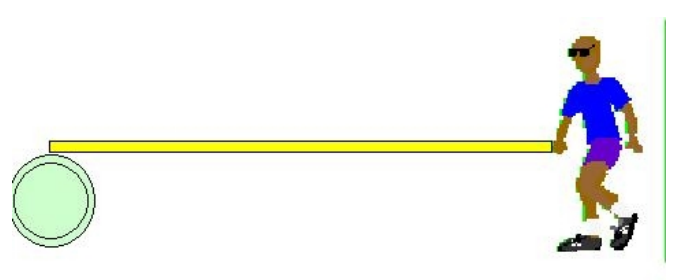
\includegraphics[width=0.5\linewidth]{2014-v3p-02-yl.PNG}
\end{center}
\fi

\ifHint
Vaadi ühe täispöördega liigub selle keskpunkt edasi vaadi ümbermõõduga võrdse teepikkuse võrra. Sama aja jooksul liigub laua vaadile toetuv ots vaadi keskpunkti suhtes edasi sama teepikkuse võrra. 
\fi

\ifSolution
Vaadi ühe täispöördega liigub selle keskpunkt edasi teepikkuse $ 2\pi  R$ võrra, kus $R$ on vaadi raadius. Sama aja jooksul liigub laua vaadile toetuv ots vaadi keskpunkti suhtes edasi sama teepikkuse võrra. Kuivõrd vaat pöörleb ja liigub ning laud liigub vaadi suhtes, liigub lauda lükkav mees selle aja jooksul edasi teepikkuse $2 \cdot 2 \pi R$ võrra, mis on kaks korda pikem kui vaadi telje poolt läbitud teepikkus. Seega, et mees jõuaks vaadini, peab ta läbima teepikkuse, mis võrdub laua kahekordse pikkusega ehk $12$ m.
\fi
}
